\documentclass[11pt,twocolumn]{ctexart} % 使用 ctexart 支持中文,添加 twocolumn 选项

% 基础数学支持
\usepackage{amsmath, amssymb, amsfonts}

% 图形和绘图支持
\usepackage{graphicx}
\usepackage{tikz}
\usepackage{pgfplots}
\pgfplotsset{compat=1.17}

% 页面设置和布局
\usepackage{geometry}
\usepackage{hyperref}

% 参考文献和引用
\usepackage{natbib}

% 图表标题支持
\usepackage{caption}
\usepackage{subcaption}

% 中文支持(ctexart已经包含了中文支持,不需要额外的xeCJK)
% 如果需要特别指定中文字体,可以使用:
% \setCJKmainfont{Microsoft YaHei}  % 设置中文字体为微软雅黑


\documentclass[11pt,twocolumn]{ctexart}
% 添加分栏线
\usepackage{multicol}
\setlength{\columnseprule}{0.4pt}  % 分栏线宽度
\setlength{\columnsep}{1cm}        % 分栏间距

% 控制浮动体
\usepackage{float}


\geometry{left=3cm, right=3cm, top=3cm, bottom=3cm}
\pgfplotsset{compat=newest}

\title{反向传播算法中负梯度在参数更新中的作用:方向与步长的详析}
\author{ChenZhuoWen}
\date{\today}

\begin{document}
\maketitle

\begin{abstract}
本报告深入探讨了反向传播算法中负梯度在参数更新过程中的核心作用。我们从数学定义出发,详细分析了梯度和方向导数的关系,并阐明了为何负梯度不仅指示了更新方向,还通过其模长决定了更新步长。通过三维图示,我们直观展示了损失函数曲面及负梯度的作用。希望本报告能帮助读者更深入地理解深度学习中梯度下降法的基本原理。
\end{abstract}

\section{引言}
反向传播算法是训练神经网络的基础,其核心在于通过计算损失函数对参数的梯度来指导参数更新。梯度下降法的更新公式为
\begin{equation}
    \boldsymbol{\theta}_{\text{new}} = \boldsymbol{\theta}_{\text{old}} - \eta \nabla L(\boldsymbol{\theta}),
\end{equation}
其中 \( L \) 为损失函数,\(\boldsymbol{\theta}\) 为参数向量,\(\eta\) 为学习率。由于梯度 \( \nabla L \) 指向损失增加最快的方向,所以取其负值 \( -\nabla L \) 则能使损失下降最快。本文将详细论述这一原理,并结合图示说明其直观意义。

\section{理论背景}
\subsection{梯度与方向导数}
设多元函数 \( f(\theta_1, \theta_2, \ldots, \theta_n) \) 在点 \(\boldsymbol{\theta}=(\theta_1,\theta_2,\ldots,\theta_n)\) 处的梯度定义为
\begin{equation}
    \nabla f(\boldsymbol{\theta}) = \left( \frac{\partial f}{\partial \theta_1},\, \frac{\partial f}{\partial \theta_2},\, \ldots,\, \frac{\partial f}{\partial \theta_n} \right).
\end{equation}
梯度向量不仅反映了函数在各方向上的变化率,其方向正是函数增值最快的方向。对于任一单位向量 \( \mathbf{v} \),函数沿该方向的方向导数为
\begin{equation}
    D_{\mathbf{v}} f(\boldsymbol{\theta}) = \nabla f(\boldsymbol{\theta}) \cdot \mathbf{v} = \|\nabla f(\boldsymbol{\theta})\| \cos \theta,
\end{equation}
其中 \(\theta\) 为 \(\nabla f(\boldsymbol{\theta})\) 与 \( \mathbf{v} \) 的夹角。

\subsection{负梯度与参数更新}
在梯度下降法中,参数更新公式为
\begin{equation}
    \Delta \boldsymbol{\theta} = -\eta \nabla L(\boldsymbol{\theta}).
\end{equation}
这里:
\begin{itemize}
    \item \textbf{更新方向}:由于梯度 \( \nabla L \) 指向损失函数上升最快的方向,因此负梯度 \( -\nabla L \) 指向损失下降最快的方向;
    \item \textbf{更新步长}:梯度的模长 \( \|\nabla L\| \) 表示函数变化的速率,乘以学习率 \( \eta \) 后决定了步长大小。
\end{itemize}
因此,负梯度在一次更新中既给出了参数改变的方向,又决定了改变的幅度。

\section{三维图示与直观分析}
为便于直观理解,我们以简单的二元函数为例:
\begin{equation}
    L(\theta_1, \theta_2) = \theta_1^2 + \theta_2^2,
\end{equation}
其梯度为
\begin{equation}
    \nabla L = (2\theta_1,\, 2\theta_2).
\end{equation}
在此例中,梯度的方向与参数 \((\theta_1,\theta_2)\) 的方向一致,而负梯度则指向原点(损失值较低的区域)。

图 \ref{fig:loss_surface} 展示了函数 \( L(\theta_1,\theta_2) \) 的三维曲面;图 \ref{fig:gradient_descent} 中,我们在点 \((1,1)\)处标出了负梯度,并用箭头展示了参数更新的方向和相对步长。

\begin{figure}[H]
    \centering
    \resizebox{0.8\columnwidth}{!}{
        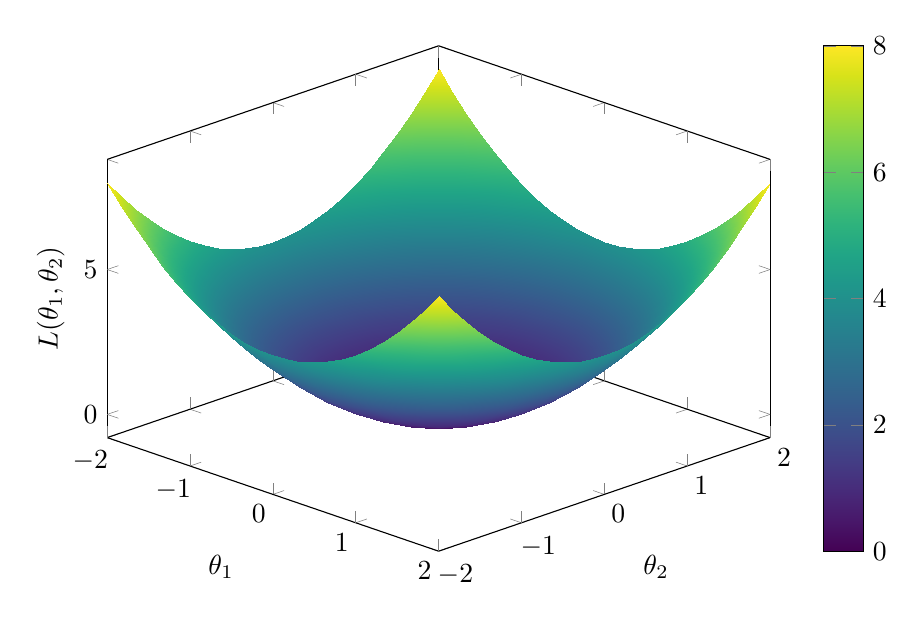
\begin{tikzpicture}
    \begin{axis}[
        width=10cm,
        height=8cm,
        view={45}{30},
        xlabel={$\theta_1$},
        ylabel={$\theta_2$},
        zlabel={$L(\theta_1,\theta_2)$},
        domain=-2:2,
        y domain=-2:2,
        colormap/viridis,
        colorbar,
    ]
    \addplot3[
        surf,
        shader=interp,
    ] {x^2 + y^2};
    \end{axis}
    \end{tikzpicture}
    
    }
    \caption{损失函数 \( L(\theta_1,\theta_2)=\theta_1^2+\theta_2^2 \) 的三维曲面图示。}
    \label{fig:loss_surface}
\end{figure}

\begin{figure}[H]
    \centering
    \resizebox{0.8\columnwidth}{!}{
        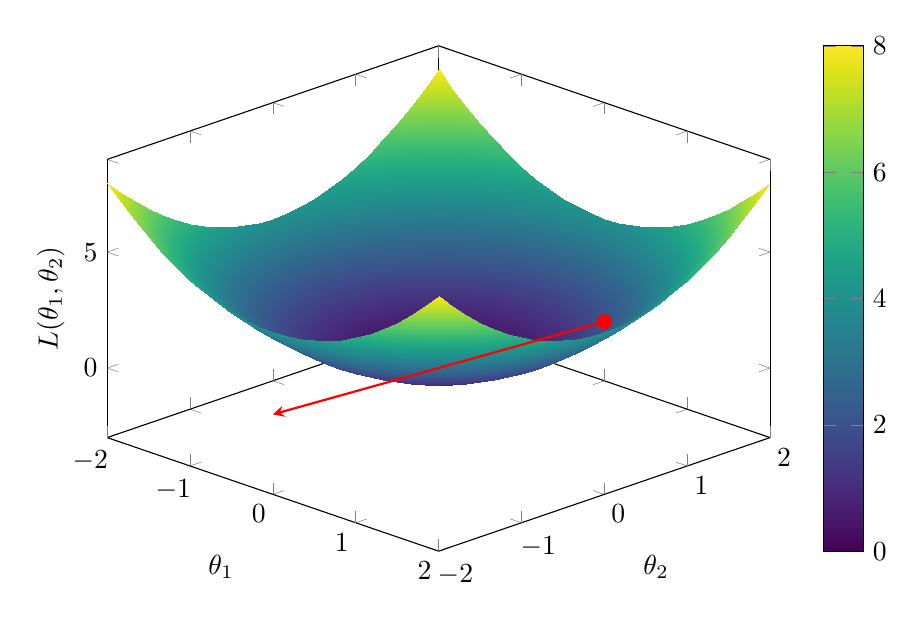
\begin{tikzpicture}
    \begin{axis}[
        width=10cm,
        height=8cm,
        view={45}{30},
        xlabel={$\theta_1$},
        ylabel={$\theta_2$},
        zlabel={$L(\theta_1,\theta_2)$},
        domain=-2:2,
        y domain=-2:2,
        colormap/viridis,
        colorbar,
    ]
    % 绘制损失函数曲面
    \addplot3[
        surf,
        shader=interp,
    ] {x^2 + y^2};
    
    % 标记一个具体点 (1,1)
    \addplot3[
        only marks,
        mark=*,
        mark options={fill=red},
        red,
        mark size=2.5pt,
    ] coordinates {(1,1,{1^2+1^2})};
    
    % 绘制负梯度向量(在点 (1,1)处计算)
    % 由于梯度为 (2*1, 2*1),负梯度为 (-2, -2)。
    % 为了在三维图中展示,我们对z方向也给定一个缩放因子,便于直观展示。
    \addplot3[
        -stealth,
        red,
        thick,
        quiver={
            u={-2},
            v={-2},
            w={-0.5*(2^2+2^2)}  % 此处w分量用于调整图示效果
        },
        domain=0:0.5,
        samples=2,
    ] coordinates {(1,1,{1^2+1^2})};
    \end{axis}
    \end{tikzpicture}
    
    }
    \caption{在点 \((1,1)\)处,红色箭头表示负梯度 \( -\nabla L \),指示了参数更新的方向与步长(由梯度模长决定)。}
    \label{fig:gradient_descent}
\end{figure}

\section{实验与讨论}
在实际神经网络训练中,损失函数往往具有更为复杂的形状(可能是非凸的),但梯度下降法仍然依靠负梯度来引导参数向局部或全局最优解更新。实际情况中,我们可能遇到以下现象:
\begin{itemize}
    \item 当损失函数变化剧烈时,梯度模长较大,更新步长也大,可能会引起震荡;
    \item 学习率的选取对平衡更新步长起到关键作用;
    \item 为提高稳定性和收敛速度,常采用动量、AdaGrad、Adam等改进的优化算法,这些方法在原始负梯度的基础上对更新进行调节。
\end{itemize}
上述讨论表明,理解负梯度在更新中的双重作用对于设计高效的优化算法至关重要。

\section{结论}
本文从数学定义和直观图示两方面详细阐述了反向传播算法中负梯度的作用。负梯度不仅为参数更新提供了明确的方向(即损失下降最快的方向),还通过梯度模长决定了更新步长。这一原理构成了梯度下降法及其改进算法的理论基础,对深度学习模型的训练起着决定性作用。

\section{未来工作}
未来的研究可以进一步探讨复杂损失函数下负梯度信息的利用,特别是在自适应优化和非凸优化问题中的应用。同时,通过更高维度的可视化方法,帮助我们更直观地理解深度网络中参数空间的结构和优化路径。

\bibliographystyle{plain}
\bibliography{references}
\end{document}
